\documentclass[handout]{beamer}

\graphicspath{{../assets/}}

\usetheme{Copenhagen}

\title{Complex Networks}
\author{Shoichi Yip}
\institute{M2 PCS}
\date{3 April 2024}

\begin{document}

\frame{\titlepage}

\section{Random graphs of the configuration model}

\begin{frame}{Random graphs}
\end{frame}

\begin{frame}{The configuration model}
\end{frame}

\begin{frame}{Our ensemble}
    In our particular case, we define a random graph ensemble $\mathcal{G}$ such
    that:
    \begin{itemize}
        \item the graph has $N$ nodes;
        \item the graph is generated using the configuration model;
        \item the graph doesn't contain self-edges and multiple edges;
        \item we define a parameter $\pi$ and the the graph is such that the
            fraction of the nodes $p_1 = 1-\pi$ has degree 1, and the remaining
            fraction $p_4 = \pi$ has degree 4.
    \end{itemize}
\end{frame}

\begin{frame}{Examples of random graphs}
    \begin{figure}
        \centering
        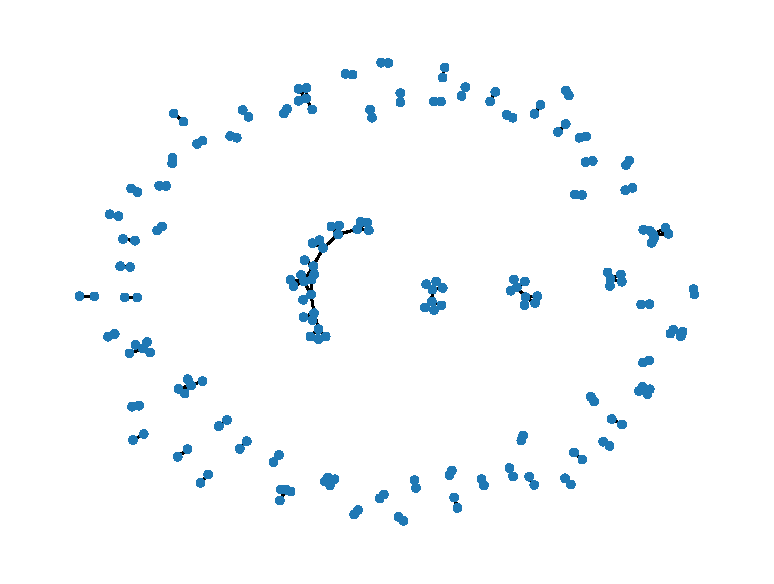
\includegraphics[height=.7\textheight]{rg0}
        \caption{Instance of a random graph for $\pi=0.1$}
        \label{fig:rg0}
    \end{figure}
\end{frame}

\begin{frame}{Examples of random graphs}
    \begin{figure}
        \centering
        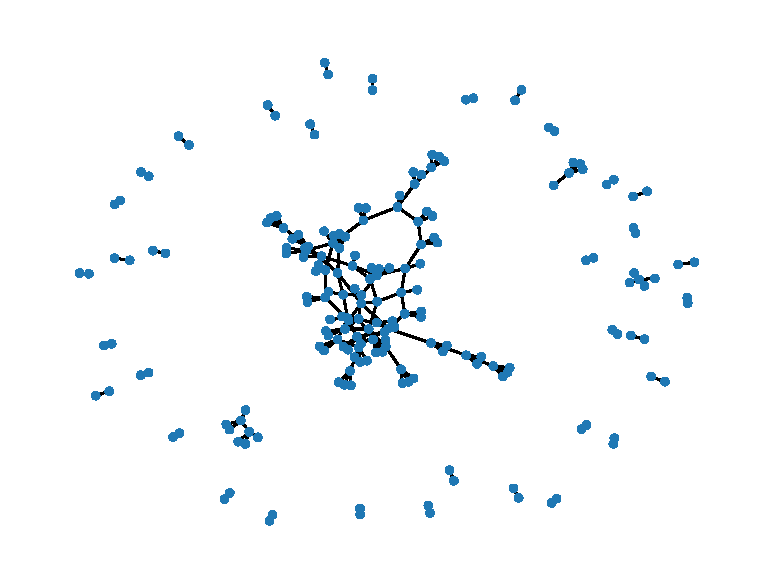
\includegraphics[height=.7\textheight]{rg1}
        \caption{Instance of a random graph for $\pi=0.3$}
        \label{fig:rg1}
    \end{figure}
\end{frame}

\begin{frame}{Examples of random graphs}
    \begin{figure}
        \centering
        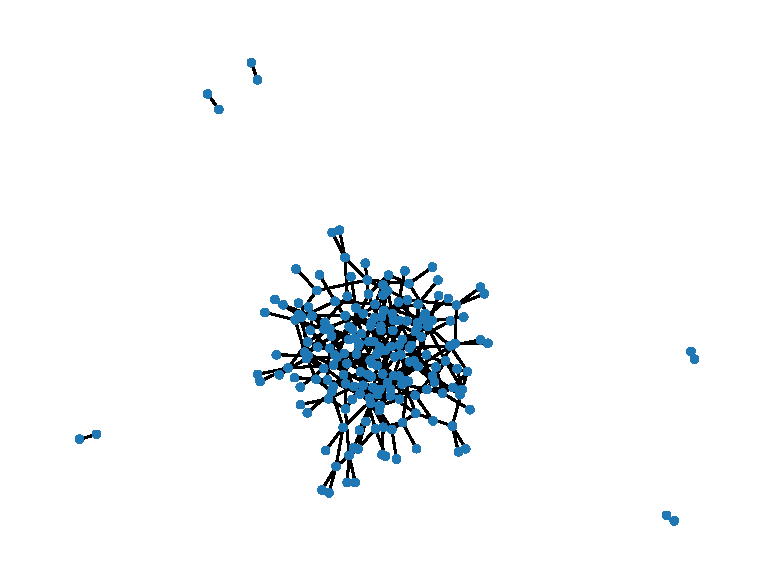
\includegraphics[height=.7\textheight]{rg2}
        \caption{Instance of a random graph for $\pi=0.7$}
        \label{fig:rg2}
    \end{figure}
\end{frame}

\section{The giant component}

\begin{frame}{The size of the giant component}
    \begin{figure}
        \centering
        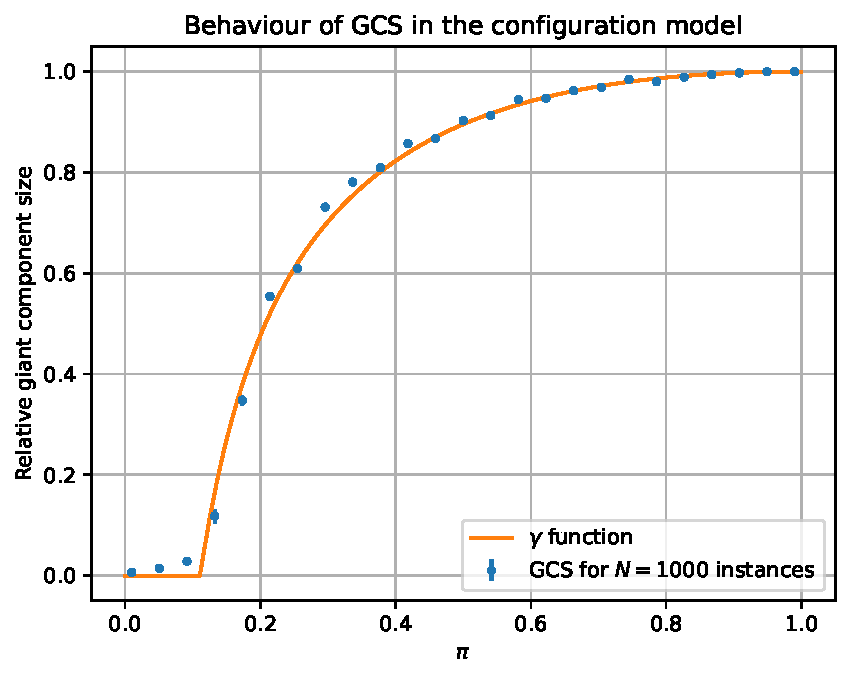
\includegraphics[height=.7\textheight]{gcs}
        \caption{Comparison between theoretical value and measures from random
        instances of the size of the giant component}
        \label{fig:gcs}
    \end{figure}
\end{frame}

\section{Emergence of $q$-cores}

\begin{frame}{The size of the 3-core}
    \begin{figure}
        \centering
        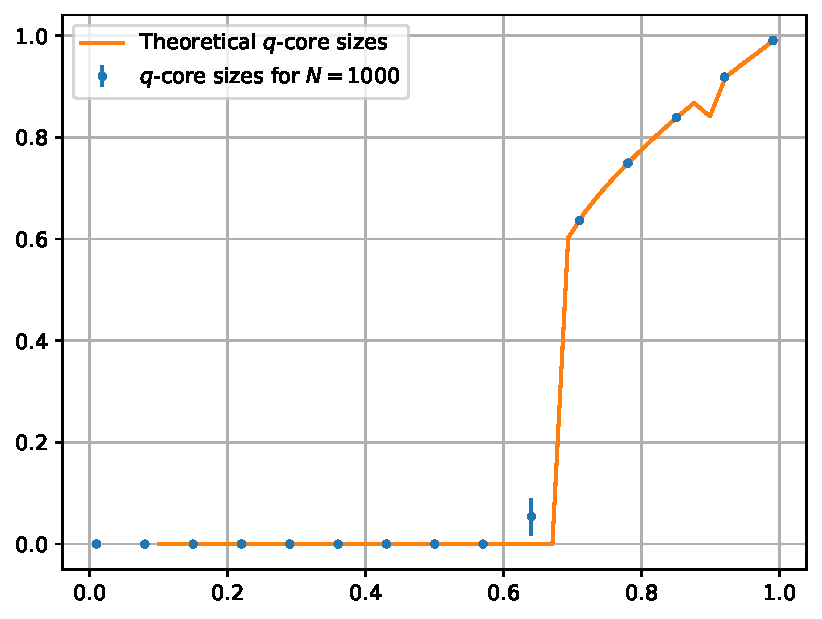
\includegraphics[height=.7\textheight]{qcore}
        \caption{Comparison between theoretical value and measures from random
        instances of the size of the 3-core}
        \label{fig:gcs}
    \end{figure}
\end{frame}

\section{The ferromagnetic Ising model}

\section{Inverse Ising model}

\end{document}
